\chapter{Results}
\label{ch:testing}

\section{Simulation parameters}

\begin{figure} [h]
\centering
\hspace*{-1.0in}
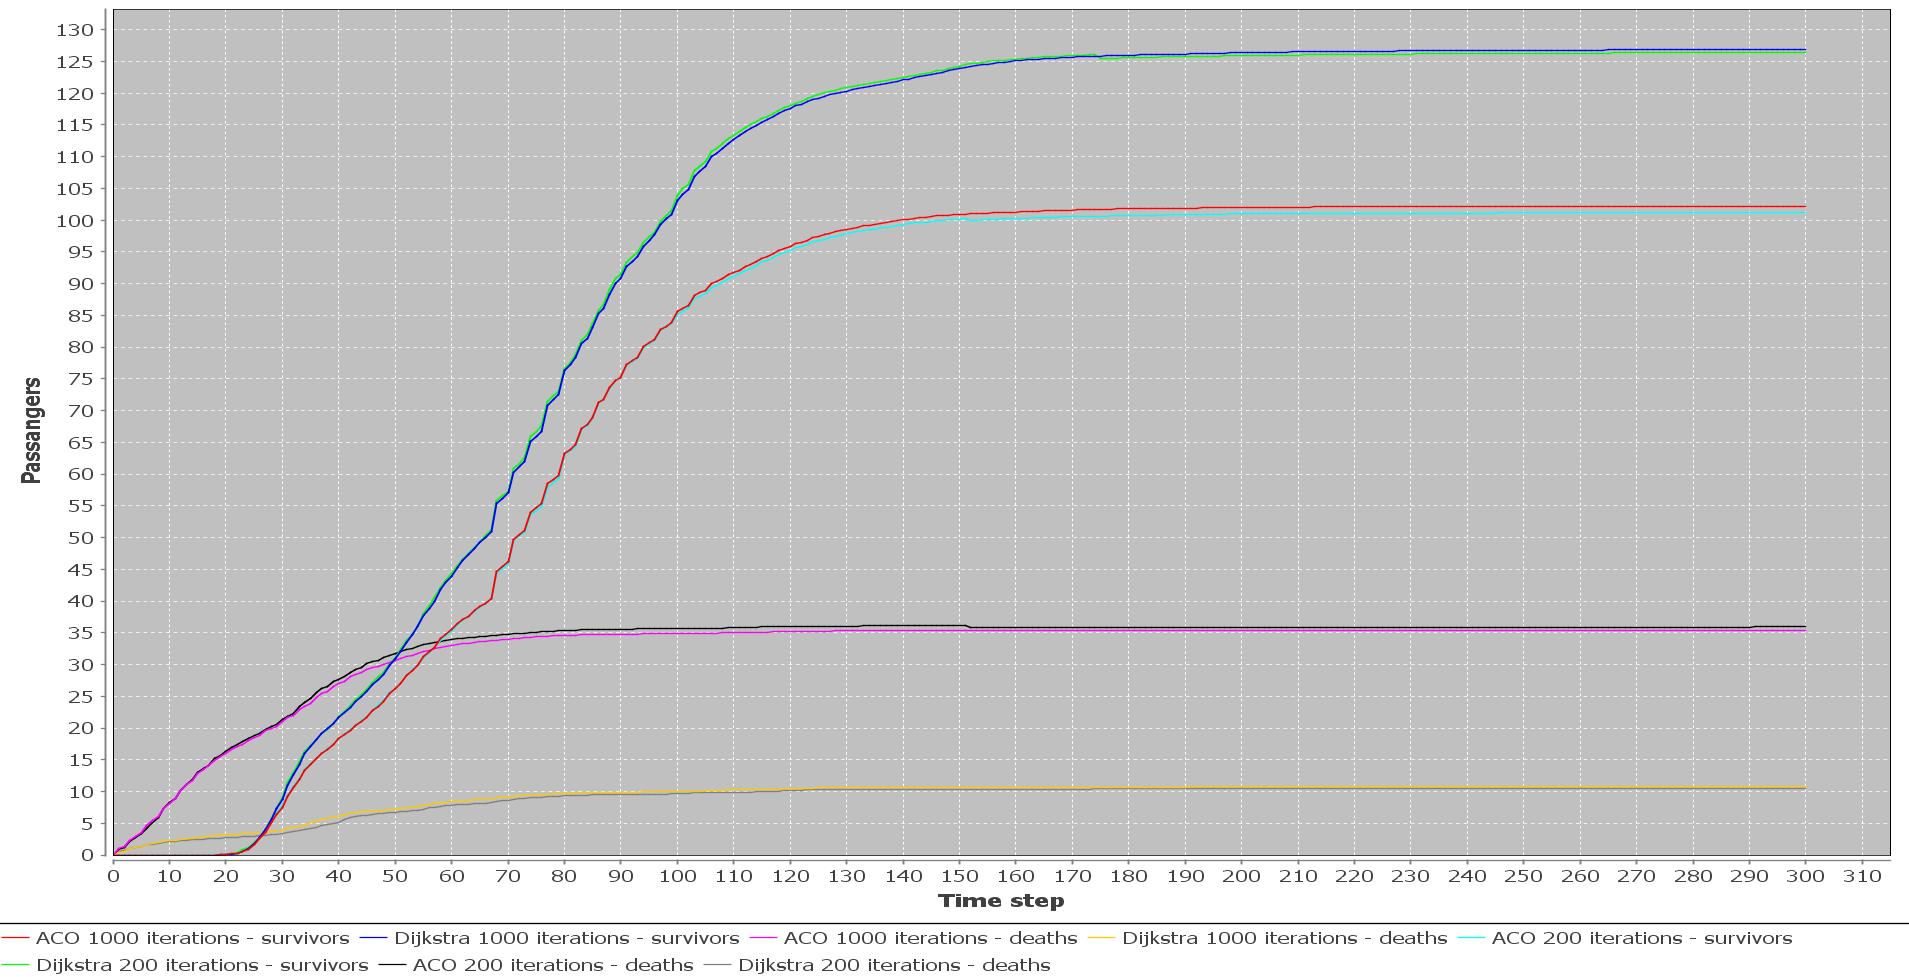
\includegraphics[scale=0.35]{images/Graph-using-200-rounds-and-1000-rounds.png}
\caption{Comparing 200 iterations to 1000 iterations.}
\label{fig:celeb1000}
\end{figure}

In the simulations there are several parameters that can be changed and multiple variables that can have an extreme impact on the simulation. For instance the fires can cover all exits and end up killing most if not all passengers. Thus each simulation runs 200 times and we obtain the average results. We found that there was no significant difference between 200 iterations and 1000 iterations, that can see in figure \ref{fig:celeb1000}.

\begin{figure} [h]
\centering
\hspace*{-1.0in}
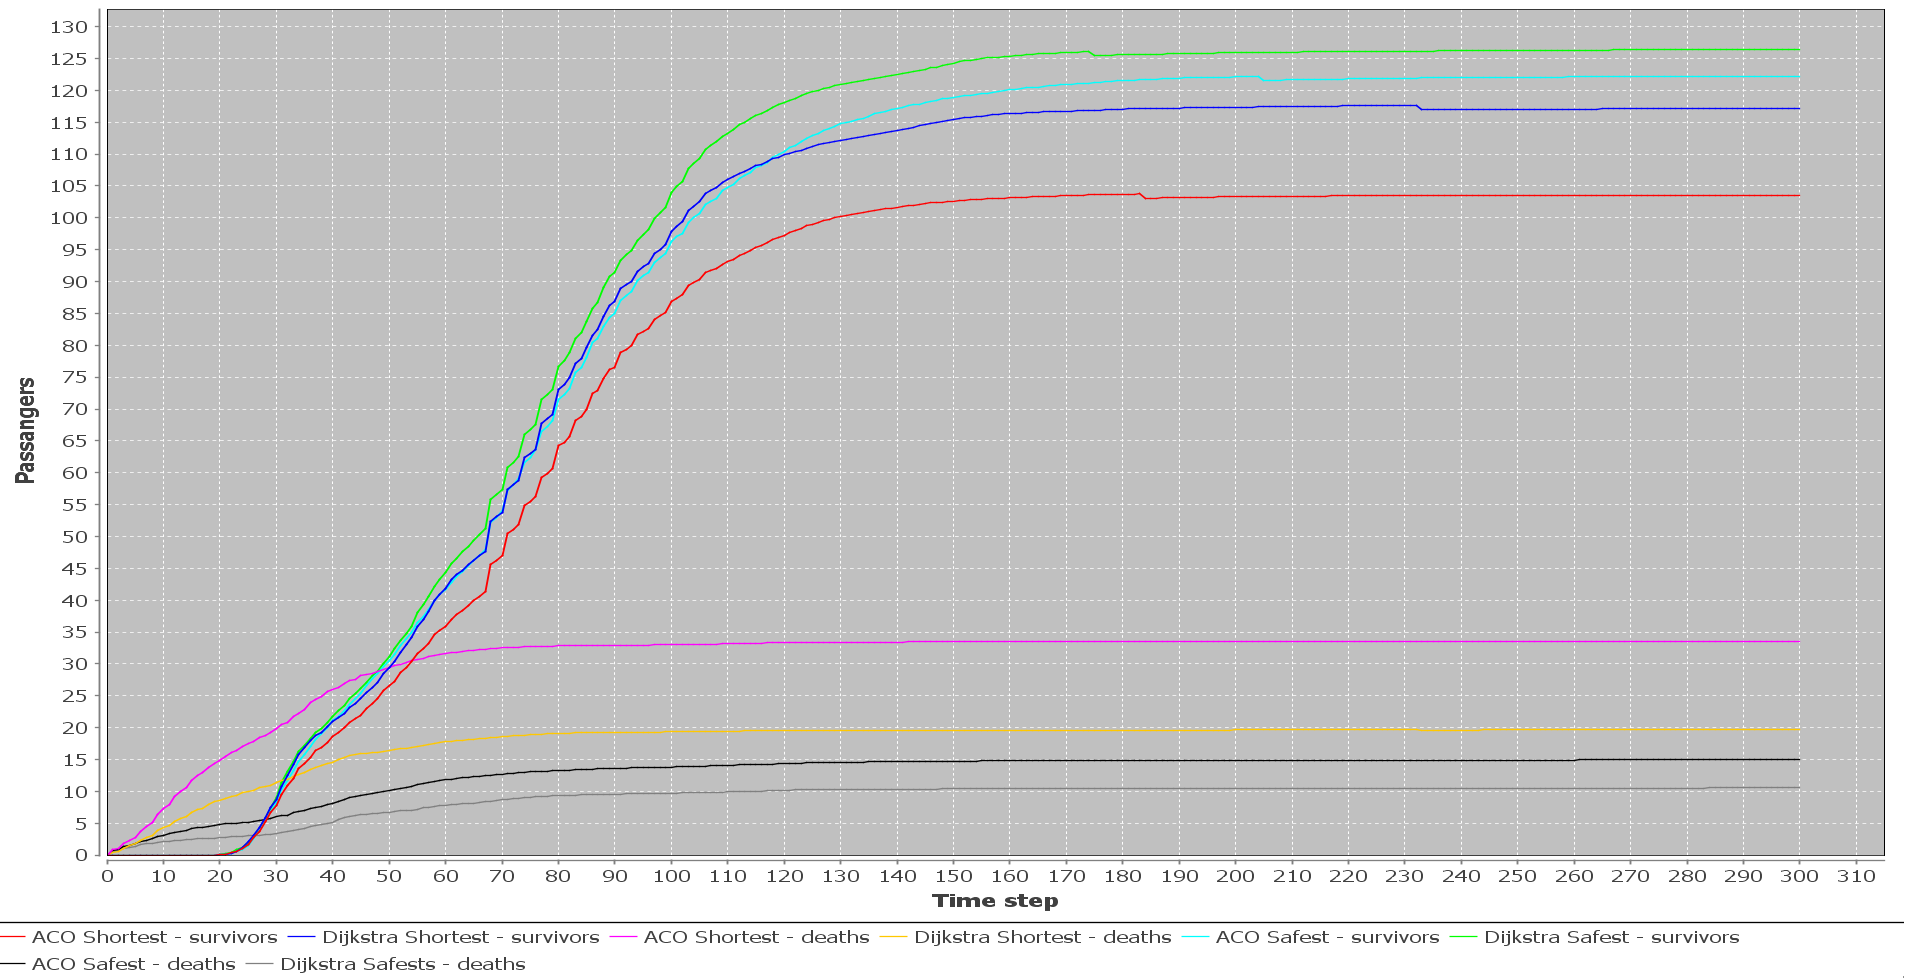
\includegraphics[scale=0.35]{images/Graph-using-200-rounds-140-passangers.png}
\caption{Dijkstra and ACO running at each time step.}
\label{fig:celeb}
\end{figure}


% Crew members not accounted for
The simulations also ran with a set of standard configurations. When the effects of changing one parameter was tested the remaining ones were kept at a standard level. The number of passengers was set to the ship maximum number of passengers used on the ship Celebrity Xpedition was found on Cruisedeckplans LLC website\cite{cruseships}. The fire on board the ship was set to increase in size and intensity at every second time step, one time step being 1-2 real life seconds. At the start of the simulations between one and three fires were started.

At each time step ACO released 200 ants per passenger. Each ant held 100 pheromones that it used to mark the paths to the exits. The passengers would use these new paths. Similarly Dijkstra's algorithm recalculated a new path for each passenger at each time step. In some of our simulation a few passenger would not reach the exits within 300 time steps. However we have cut the graph at 300 time steps, as this would show more details in the graph and the average number of survivors past 300 did not change. 


\section{Testing}

\begin{figure} [h]
\centering
\hspace*{-1.0in}
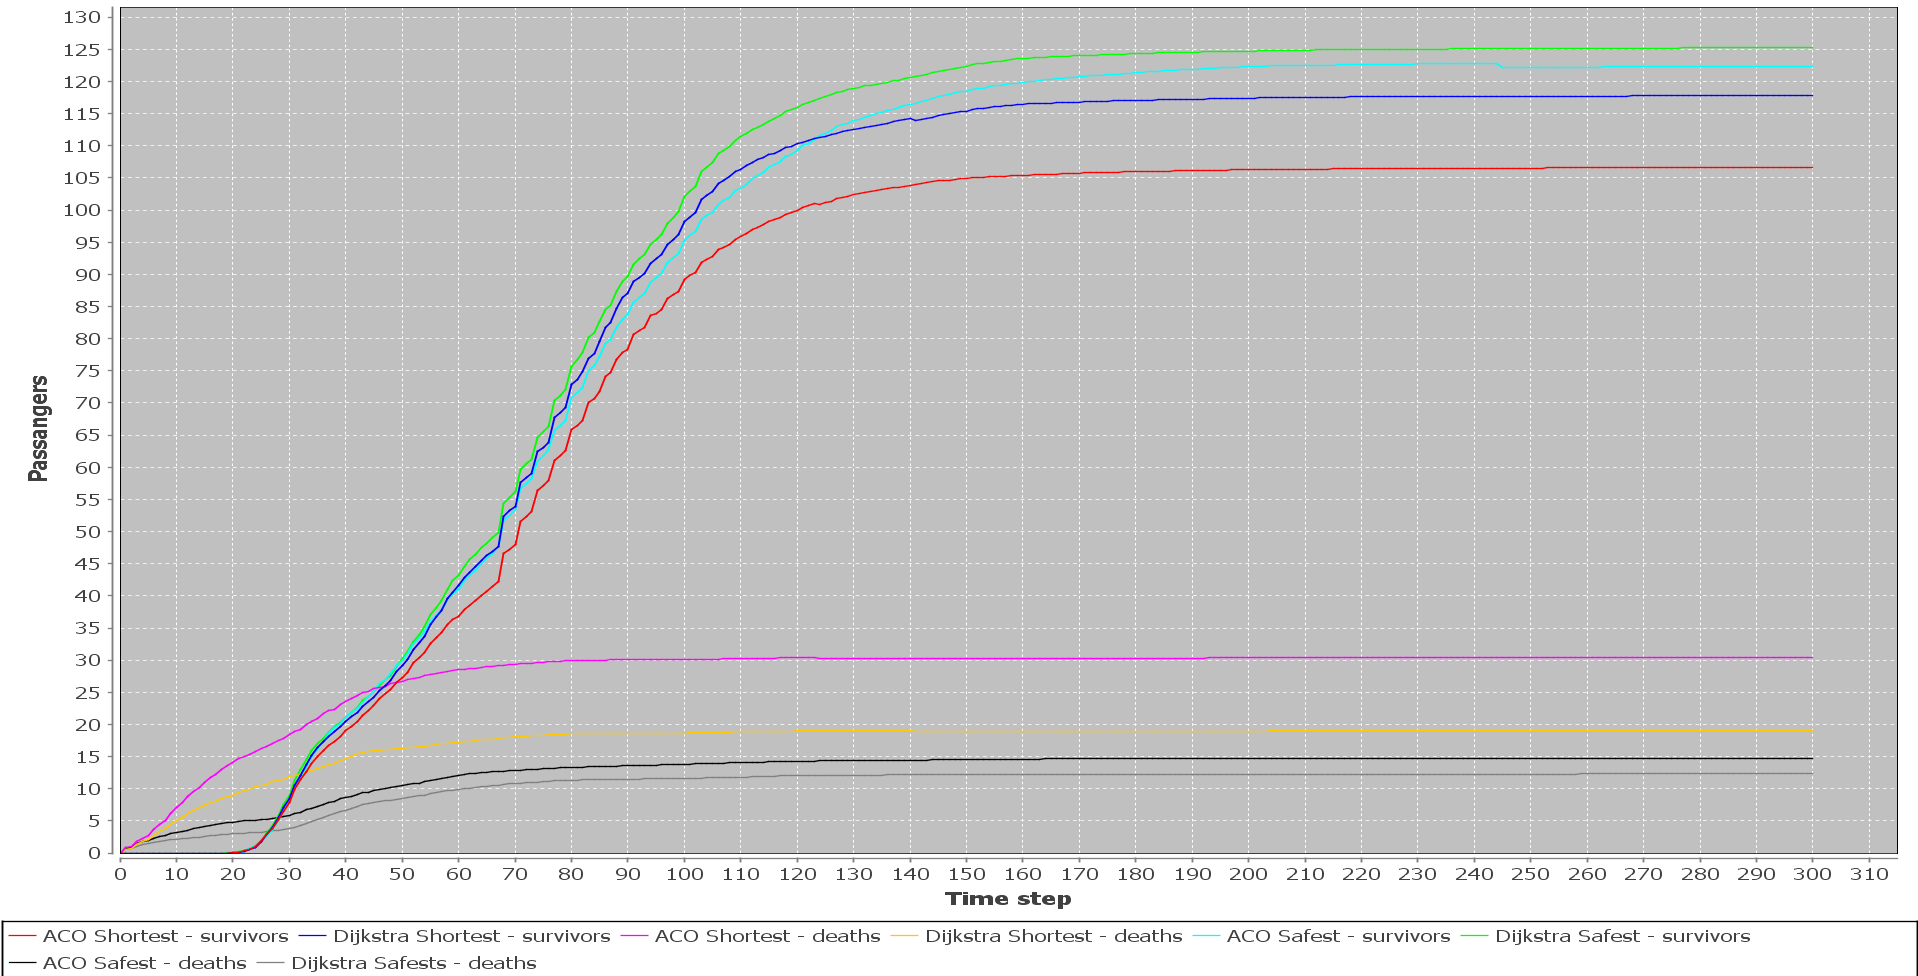
\includegraphics[scale=0.35]{images/Graph-using-200-rounds-140-passangers-and-ACO-having-pheremons-in-edges.png}
\caption{Taking shortest path with pheromones in edges.}
\label{fig:celebPherInEdge}
\end{figure}
\subsection{Pheromones in edges}

At the beginning of the testing phase we tested whether ants depositing pheromones in the edges or in the nodes gave the best results.  As seen in figure \ref{fig:celebPherInEdge} tests showed depositing pheromones in the nodes performed equal to depositing pheromones in the edges when searching for the safest path, however when ACO was trying to search for the quickest path depositing pheromones in the edges provided better results. Thus we decided to keep depositing pheromones this way for all future tests.

\subsection{Dijkstra's algorithm}

In figure \ref{fig:celebDF} we see the results of running Dijkstra's algorithm once per passenger at the start of the simulation and no more as the simulation progressed. When searching for the safest path we expected that ACO would outperform Dijkstra's algorithm, and it did. When Dijkstra's algorithm could not account for the fire spreading its performance suffered. When looking for the shortest path, ACO started out well but Dijkstra's algorithm caught up after about 100 time steps. This shows that people are exiting the dangerous area faster with ACO but the two algorithms performance regarding survivors is almost identical.

\begin{figure} [h]
\centering
\hspace*{-1.0in}
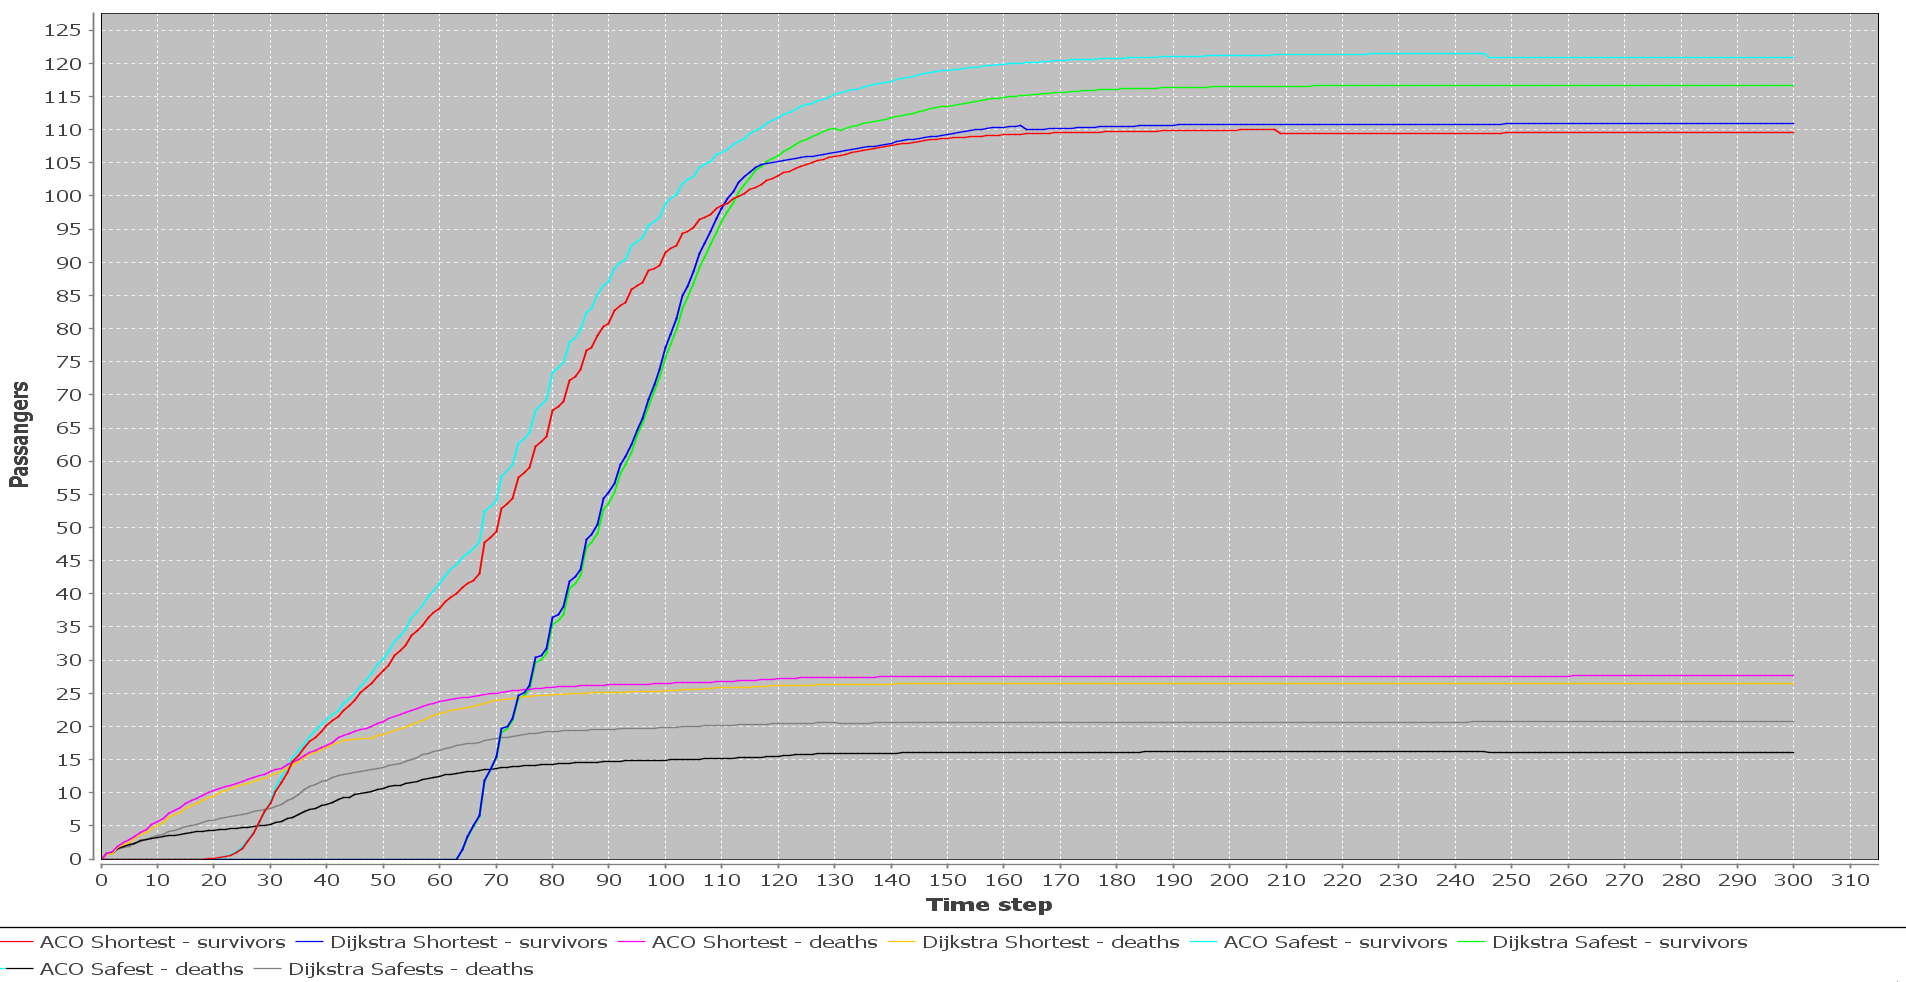
\includegraphics[scale=0.35]{images/Graph-using-200-rounds-140-passangers-and-dijkstra-one-time.png}
\caption{Running Dijkstra's algorithm only at start.}
\label{fig:celebDF}
\end{figure}

In figure \ref{fig:celeb} Dijkstra's algorithm was run with the standard configurations. It is clearly seen that Dijkstra's algorithm selecting the safest path has the best results overall, however only with a slight margin. If you look at quickest paths only, it is clearly shown that ACO's passengers are dying more rapidly then Dijkstra's passengers. This means that both algorithms are choosing different paths. As the shortest path is measured in shortest time needed to reach the exit rather than the shortest distance to exit, it would seem that Dijkstra's algorithm is more effective at spreading the passengers than ACO. Additionally Dijkstra's algorithm is able to guide passengers to an exit faster than ACO.

What is clear is that selecting the safest path is the best option regardless of algorithm. This can be attributed to the speed of the passengers and speed of the fire. If the fire spread was faster and passengers moved slower then the long and safe path around the fires could lead to the fire spreading to cover the previously safe path. Which in turn could cause more lives to be lost compared to if they took the shorter and slightly more dangerous path at the start.

%you can see how well the different algorithms did. In both cases we only used one hazard(Fire) that spread on board the ship. As shown in the graph, Dijkstra outperforms ACO in both early and late stages of this graph. In the beginning there are more passengers dying to ACO chosen path then there is in Dijkstra's chosen path, a good sign that both are finding different paths. As shortest path is measured in shortest time needed rather then shortest way to exit, it may be that Dijkstra spread the passengers more out then ACO.

%Even when more passengers are dying at the beginning of the simulations, they both have the same boost in saved passengers at each time step. The biggest problem for ACO over Dijkstra is avoiding the hazards. Shown in the graph you can see that the death toll for ACO increases faster then Dijkstra's death toll.

%In \ref{fig:celeb}, we are using the same parameters as the first one, only difference is that we are looking after the safest path rather then the shortest path for the passengers. It is clearly shown that the death toll on the passengers is far lower then the previous one. However Dijkstra proves yet again to outperform ACO in this instance. After about 30 time steps Dijkstra starts to pull ahead of ACO in number of passengers it have guided to the lifeboats. Even in number of deaths it is shown that Dijkstra is better at avoiding them. If you look at Dijkstra in both cases, the number of deaths when looking after the safest path is 50\% less when looking for the shortest path. As mention earlier that the number of rounds above 200 did not matter may be shown in the two graphs below, both of them have the same set of parameters, only to have 1000 iteration instead of 200.

%In \ref{fig:celebShortPherInEdges} and \ref{fig:celebSafePherInEdges} we tested what would the difference be if we used pheromones in edges rather then in the node themselves, this showed that the ACO preformed better then our other simulations. It was compared to Dijkstra to control that there was not something special happening. The main difference is when looking for the shortest path rather then the safest. When looking for the safest there are only some small difference in both simulations.



\begin{figure} [h]
\centering
\hspace*{-1.0in}
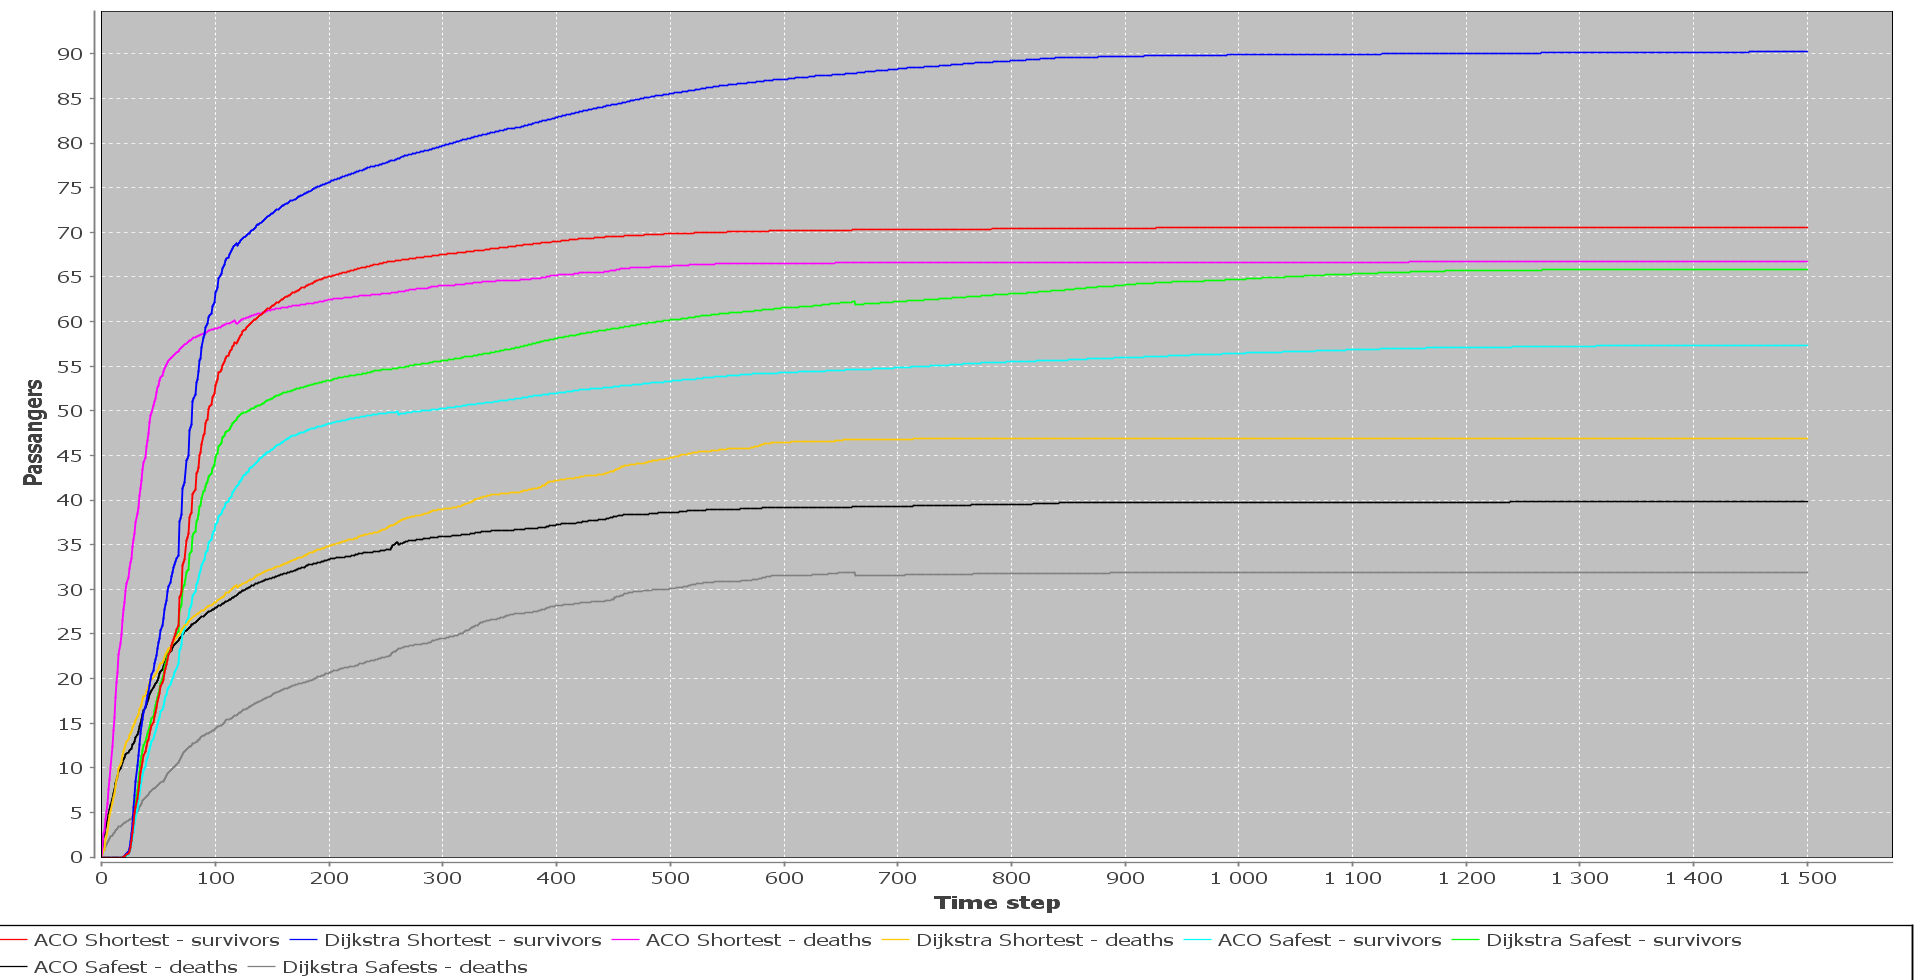
\includegraphics[scale=0.35]{images/Graph-using-200-rounds-140-passangers-and-high-panic.png}
\caption{Simulation with a high panic chance.}
\label{fig:celebHPanic}
\end{figure}

\subsection{Higher chance of panic}

When the chance of panic was increased both algorithms struggled more to guide the passengers to safety, as seen in figure \ref{fig:celebHPanic}. Dijkstra's algorithm had the largest drop in performance. In general it would seem that taking the shortest path out was the best solution as it would give the passenger the least amount of time to panic. When trying to guide the passengers through the longer, and beforehand believed to be the safest, path passengers would panic and stop following directions before reaching the exit. It is not shown in this graph but ACO spent aproximately 2400 time steps to guide the passengers out while Dijkstra's algorithm spent over 600 000 time steps to finish the simulation. While Dijkstra's algorithm had the best results of the different configurations when searching for the shortest path it also had the worst results when searching for the safest path.

\begin{figure} [h]
\centering
\hspace*{-1.0in}
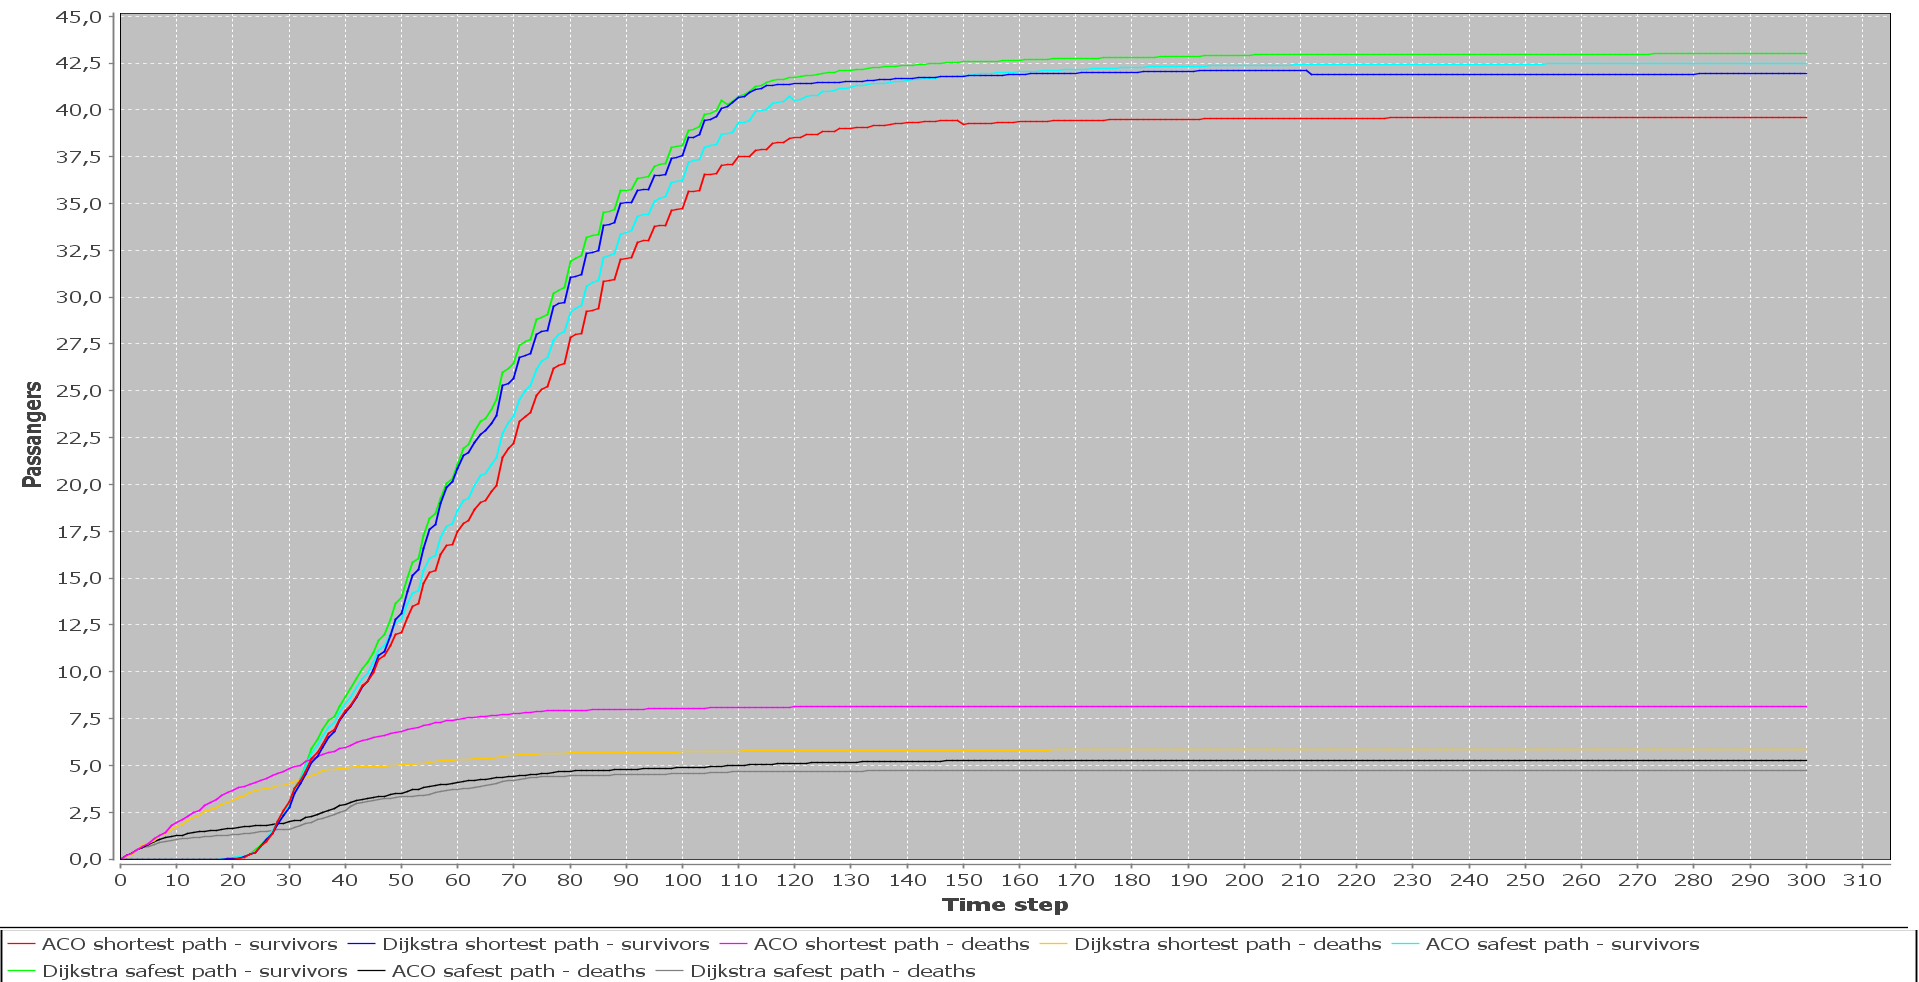
\includegraphics[scale=0.35]{images/Graph-using-200-rounds-50-passangers.png}
\caption{Simulation run with below half passenger capacity.}
\label{fig:celeb50}
\end{figure}

\begin{figure} [h]
\centering
\hspace*{-1.0in}
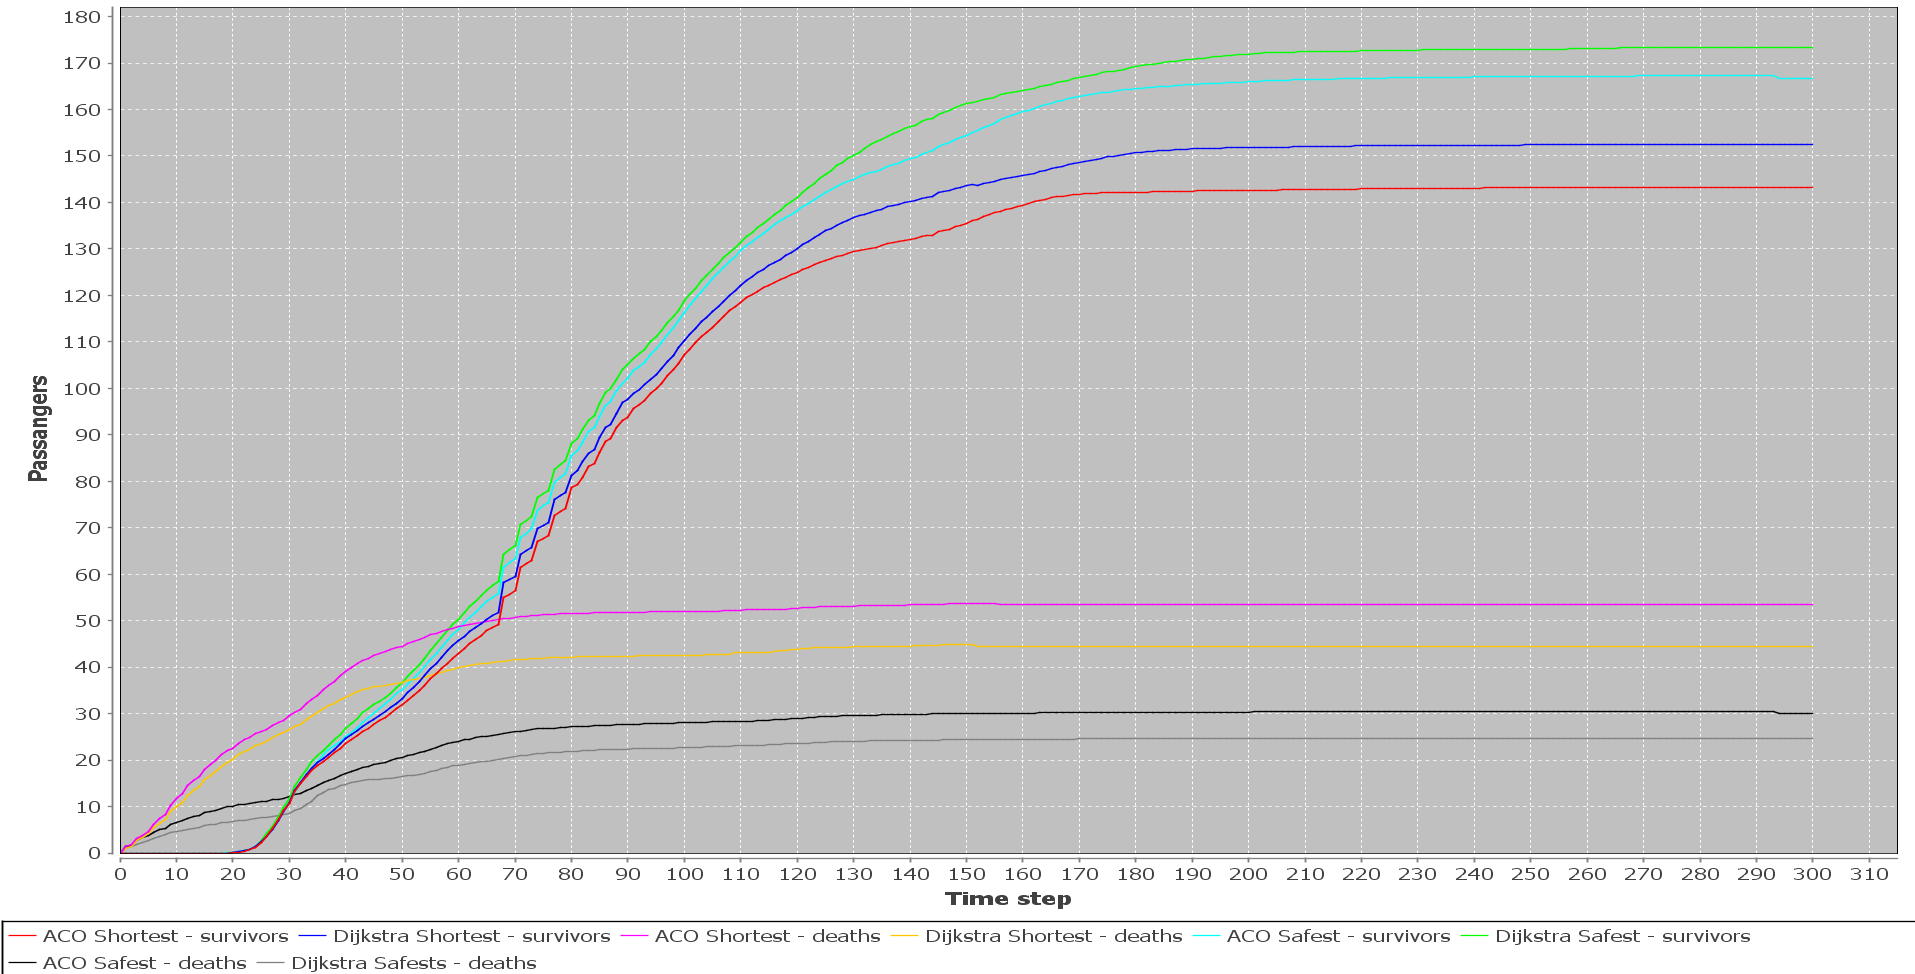
\includegraphics[scale=0.35]{images/Graph-using-200-rounds-200-passangers.png}
\caption{Simulation run with over maximum passenger capacity.}
\label{fig:celeb200}
\end{figure}

\subsection{Varying amount of passengers}

In figure \ref{fig:celeb50} all the different algorithms performance are similar and they produce better results when there are less passengers on board the ship. The order of which algorithm performs the best still remains the same. This is as expected as fewer passengers means a reduced chance of congestion and panic. 

Now in figure \ref{fig:celeb200} one can observe a larger difference in performance between the algorithms and path selections compared to in figure \ref{fig:celeb50}. This shows that the more passengers the ships have, selecting the shortest path become less viable.

\begin{figure} [h]
\centering
\hspace*{-1.0in}
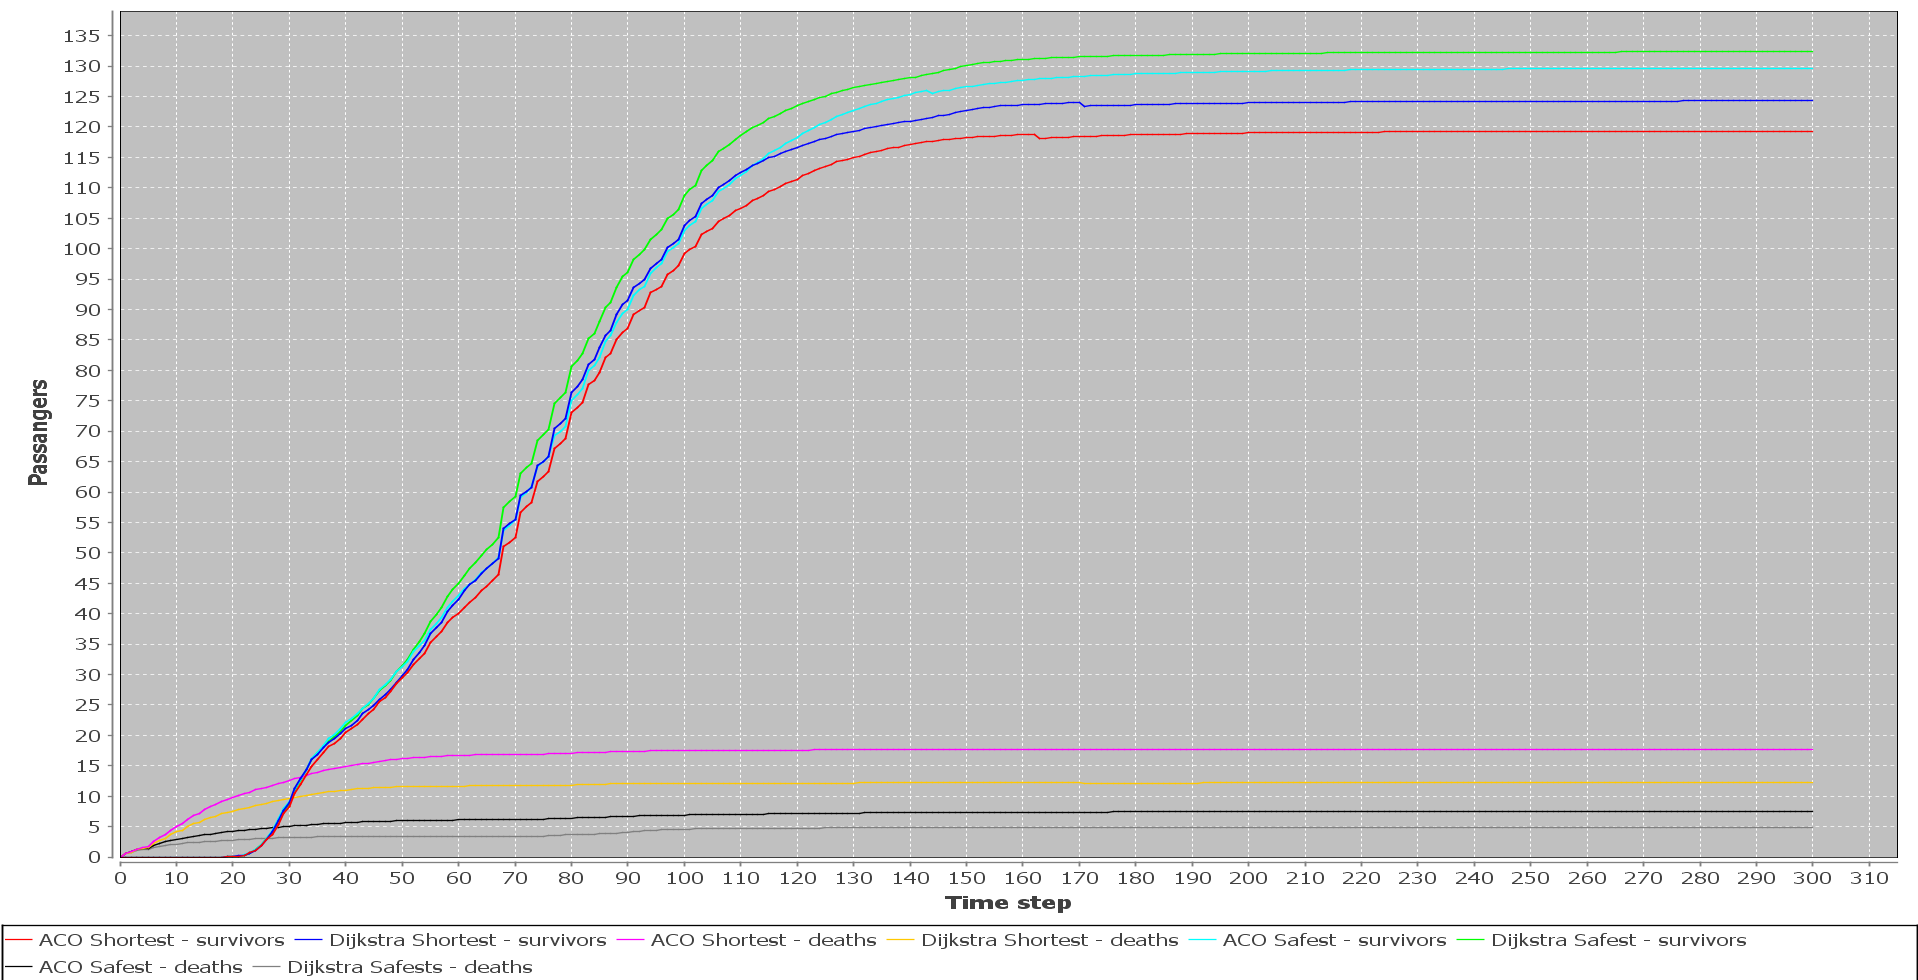
\includegraphics[scale=0.35]{images/Graph-using-200-rounds-140-passangers-slow-fire.png}
\caption{The effect of slow moving fire.}
\label{fig:celebSfire}
\end{figure}

\begin{figure} [h]
\centering
\hspace*{-1.0in}
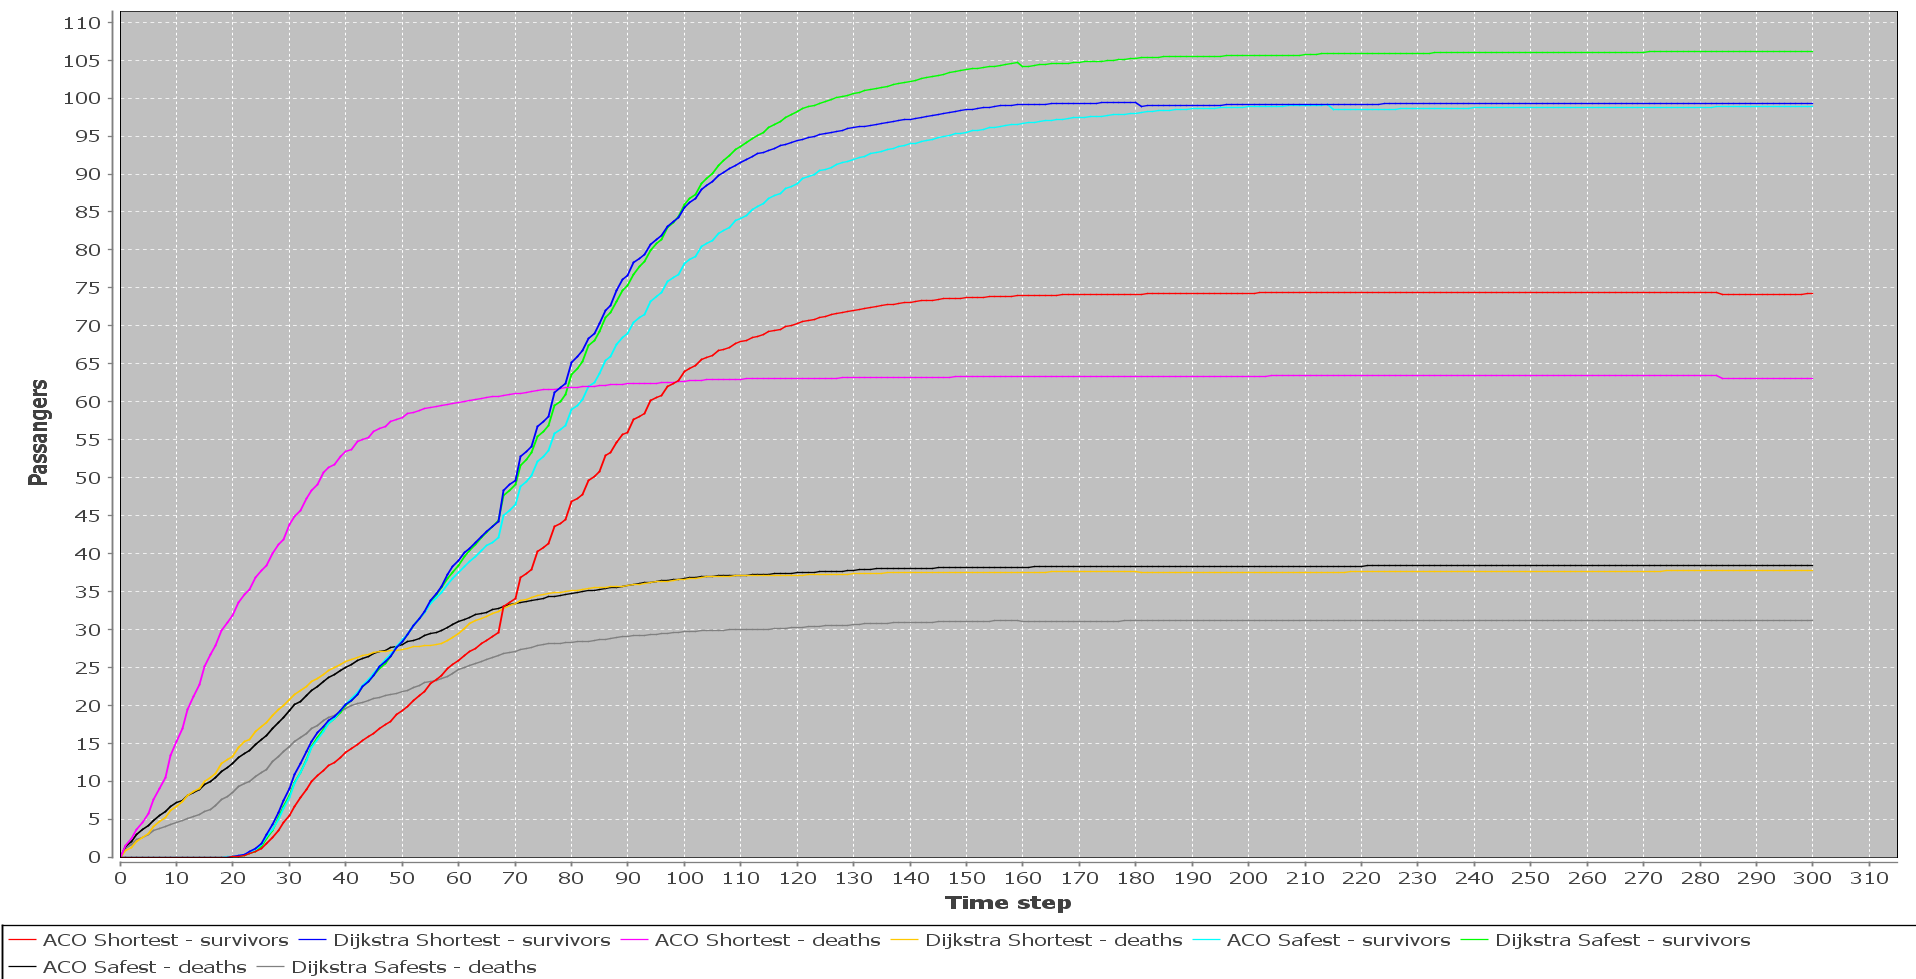
\includegraphics[scale=0.35]{images/Graph-using-200-rounds-140-passangers-and-fast-fire.png}
\caption{The effect of fast moving fire.}
\label{fig:celebFfire}
\end{figure}

\subsection{Fire spread}

In figure \ref{fig:celebSfire} the speed of the fire was decreased by 150 percent and when comparing the results to those in to figure \ref{fig:celeb} the algorithms performed better. This was expected as the hazards moved slower than in all the other simulations. It is also worth noting that when finding the quickest path ACO had the largest increase in performance, however it is still the one that is the worst off.

In figure \ref{fig:celebFfire} the speed of the fire was increased by 100 percent and all the algorithms performed worse. An interesting thing to notice in the graph is that Dijkstra searching for the shortest path is just as good as ACO searching for the safest. This shows that when the fire is spreading fast on board the ship it is not a bad idea to guide the passengers as fast as possible to an exit  as most of the escape routes are likely still viable at the start.

\begin{figure} [h]
\centering
\hspace*{-1.0in}
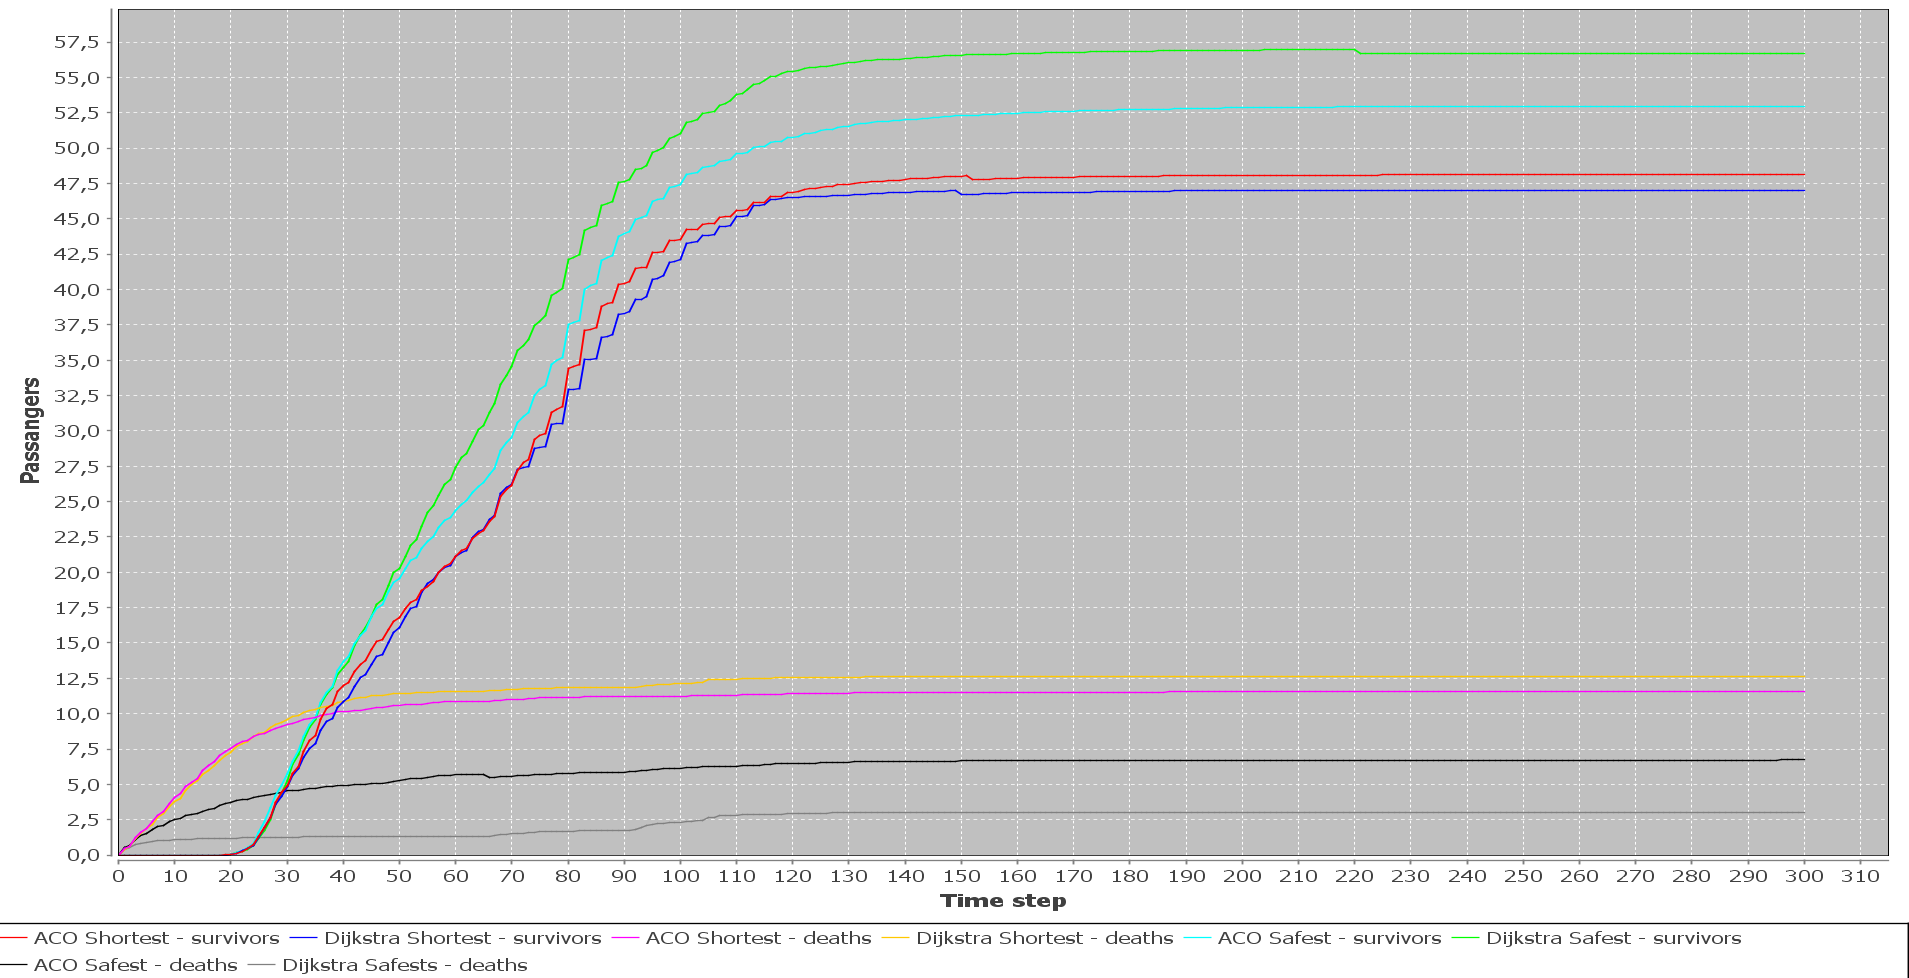
\includegraphics[scale=0.35]{images/Graph-ship-two-60-passangers-200-rounds.png}
\caption{ACO and Dijkstra's performance on Silver Explorer.}
\label{fig:silverExplor}
\end{figure}

\subsection{Second ship: Silver Explorer}
The second ship we did simulations on were the Silver Explorer. As we did not model all the floors for this ship the maximum number of passengers was not used. We used 60 passengers in this simulation, which was right below half of the maximum number disclosed on Cruisedeckplans LLC website\cite{cruseships}.

The results of this simulation can be seen in figure \ref{fig:silverExplor} and they were similar to the previous simulations, with Dijkstra's algorithm outperforming ACO slightly. Differences in performance compared to simulations made on the Celebrity Xpedition can be attributed to Silver Explorer having a different layout thus warranting a different graph that has a new set of paths.

\section{Summary of results}

Table \ref{table:tableSafest} and table \ref{table:tableShortest} shows a summary of the algorithms performance using different configurations. All the algorithms performed best in the slow moving fire simulation and they performed the worst in high panic simulation.

 Out of the simulation on Celebrity Xpedition and Silver Explorer, the Silver Explorer did the best, however the Silver Explorer was not modelled fully out as Celebrity Xpedition.

Running 200 iterations seems to be sufficient in our simulation shown by the first graph. How fast a fire was moving on board the ship had a big impact on how well the algorithms preformed for the better or worse. Having less or more passengers did not seem to affect the different algorithms to a big degree. Now having stored the pheromones in the edges of the nodes seems to be the better option then having it stored in the nodes themselves.

ACO seems to be almost just as good as Dijkstra in most cases, however when more dynamic elements are introduced into the fold ACO is much faster then Dijkstra in guiding the passengers, when looking at the high panic simulation.


\begin{table}[ht]
\caption{Survivors of safest path} 				% title of Table
\centering										% used for centering table
\begin{tabular}{c c c c}						% centered columns (4 columns)
\hline
\hline 											%inserts double horizontal lines
Case & ACO & Dijkstra \\[0.5ex]% inserts table
												%heading
\hline											% inserts single horizontal line
Standard configuration & 122,19 - (87\%) & 126,53 - (90\%) \\
Slow fire & 129,63 - (92\%) & 132,37 - (94\%) \\
Fast fire & 98,85 - (71\%) & 106,12 - (76\%) \\
High panic & 57,34 - (41\%) & 65,88 - (47\%) \\
Dijkstra only at start & 120,42 - (86\%) & 116,44 - (83\%) \\
Pheromones stored in edges & 122,31 - (87\%) & 125,25 - (89\%) \\
1000 iterations & 122,76 - (88\%) & 126,86 - (91\%) \\
50 Passengers & 42,47 - (85\%) & 43,00 - (86\%) \\
200 Passengers & 166,68 - (83\%) & 173,30 - (87\%) \\ 
Silver Explorer & 52,96 - (88\%) & 56,70 - (94\%) \\ [1ex]						% [1ex] adds vertical space
\hline														%inserts single line

\end{tabular}
\label{table:tableSafest}								
\end{table}


\begin{table}[ht]
\caption{Survivors of shortest path} 				% title of Table
\centering										% used for centering table
\begin{tabular}{c c c c}						% centered columns (4 columns)
\hline
\hline 											%inserts double horizontal lines
Case & ACO & Dijkstra \\[0.5ex]% inserts table
												%heading
\hline											% inserts single horizontal line
Standard configuration & 103,54 - (74\%) & 117,14 - (84\%)\\
Slow fire & 119,30 - (85\%) & 124,31 - (89\%) \\
Fast fire & 74,19 - (53\%) & 99,39 - (71\%) \\
High panic & 70,58 - (50\%) & 90,24 - (64\%) \\
Dijkstra only at start & 109,52 - (78\%) & 110,84 - (79\%) \\
Pheromones stored in edges & 106,58 - (76\%) & 117,80 - (84\%) \\
1000 iterations & 102,21 - (73\%) & 114,70 - (81\%) \\
50 Passengers & 39,57 - (79\%) & 41,91 - (83\%) \\ 
200 Passengers & 143,19 - (71\%) & 152,45 - (76\%) \\
Silver Explorer & 45,26 - (75\%) & 47,87 - (80\%) \\ [1ex]						% [1ex] adds vertical space
\hline														%inserts single line

\end{tabular}
\label{table:tableShortest}								
\end{table}